
\section{Relationship with local and global spectral graph partitioning}
\label{sxn:local-partitioning}
\vspace{-2mm}

In this section, we briefly describe the connections between our results 
and global and local versions of spectral partitioning, which were a 
starting point for this work.

The idea of spectral clustering is to approximate the best partition of the 
vertices of a connected graph into two pieces by using the nontrivial 
eigenvectors of a Laplacian (either the combinatorial or the normalized
Laplacian).  
This idea has had a long history~\cite{Donath:1973,fiedler75B,spielman96_spectral,guatterymiller98,ShiMalik00_NCut}.
The simplest version of spectral clustering involves computing the first 
nontrivial eigenvector (or another vector with Rayleigh quotient close to 
that of the first nontrivial eigenvector) of $L$, and ``sweeping'' over 
that vector. 
For example, 
one can take that vector, call it $x$, and, for a given threshold $K$, 
define the two sets of the partition as
\vspace{-2mm}
\begin{align*}
  C(x,K)      &= \{ i : x_i \ge K \}, \quad \text{and} \\
  \bar C(x,K) &= \{ i : x_i < K \}.
\end{align*}
Typically, this vector $x$ is computed by calling a black-box solver, but it 
could also be approximated with an iteration-based method (such as the Power
Method or Lanczos Method) or a random walk-based method (such as running a 
diffusive procedure or PageRank-based procedure to the asymptotic state).
Far from being a ``heuristic,'' 
this procedure provides a \emph{global 
partition} that (via Cheeger's inequality and for an appropriate choice of 
$K$) satisfies provable quality-of-approximation guarantees with respect to 
the combinatorial optimization problem of finding the best ``conductance'' 
partition in the entire 
graph~\cite{Mihail,spielman96_spectral,guatterymiller98}.

Although spectral clustering reduces a graph to a single vector---the 
smallest nontrivial eigenvector of the graph's Laplacian---and then 
clusters the nodes using the information in that vector, 
it is possible to obtain much more information about the graph by looking 
at more than one eigenvector of the Laplacian.  
In particular, the elements of the pseudoinverse of the combinatorial 
Laplacian, $L_0^{+}$, give local (\emph{i.e.}, node-specific) information 
about random walks on the graph.
The reason is that the pseudoinverse $L_0^+$  of the Laplacian is closely 
related to random walks on the graph.  
See, \emph{e.g.}~\cite{chebotarev1998proximity} for details.  
For example, 
it is known that the
quantity $L_0^{+} (u,u) + L_0^{+} (v,v) - L_0^{+} (u,v) - L_0^{+} (v,u)$ is
proportional to the commute time, a symmetrized version of the length of 
time before a random walker started at node $u$ reaches node $v$, whenever 
$u$ and $v$ are in the same connected component~\cite{chandra1989electrical}.  
Similarly, the elements of the pseudoinverse of the \emph{normalized} 
Laplacian give degree-scaled measures of proximity between the nodes of a 
graph.
It is likely that $L^{+}(u,v)$ has a probabilistic interpretation in terms 
of random walks on the graph, along the lines of our methodology, but we 
are not aware of any such interpretation.
From this perspective, given $L^{+}$ and a cutoff value, $K$, we can 
define a \emph{local partition} around node $u$ via 
$P_K(u) = \{ v : L^{+}(u,v) > K \}$.  
(Note that if $v$ is in $P_K(u)$, then $u$ is in $P_K(v)$; in addition, if 
the graph is disconnected, then there exists a $K$ such that $u$ and $v$ 
are in the same connected component iff $v \in P_K(u)$.)  
We call clustering procedures based on this idea \emph{local spectral 
partitioning}.

Although the na\"{i}ve way of performing this local spectral partitioning, 
\emph{i.e.}, to compute $L^{+}$ explicitly, is prohibitive for anything but 
very small graphs, these ideas form the basis for very fast local spectral 
clustering methods that employ truncated diffusion-based procedures to 
compute localized vectors with which to partition.
For example, this idea can be implemented by performing a diffusion-based 
procedure with an input seed distribution vector localized on a node $u$ and 
then sweeping over the resulting vector.
This idea was originally introduced in~\cite{Spielman:2004} as a 
diffusion-based operational procedure that was local in a very strong sense 
and that led to Cheeger-like bounds analogous to those obtained with the 
usual global spectral partitioning; and this was extended and improved 
by~\cite{andersen06local,Chung07_heatkernelPNAS}.
In addition, an optimization perspective on this was provided 
by~\cite{MOV09_TRv2}.
Although~\cite{MOV09_TRv2} is local in a weaker sense, it does obtain local 
Cheeger-like guarantees from an explicit locally-biased optimization 
problem, and it provides an optimization ansatz that may be interpreted as 
a ``local eigenvector.''
See~\cite{Spielman:2004,andersen06local,Chung07_heatkernelPNAS,MOV09_TRv2} 
for details.
Understanding the relationship between the ``operational procedure versus
optimization ansatz'' perspectives was the origin 
of~\cite{MO11-implementing} and thus of this work.


\vspace{-2mm}
\section{Heuristic justification for the Wishart density}
\label{sxn:justification}
\vspace{-2mm}

In this section, we describe a sampling procedure for $L$ which, in a very 
crude sense, leads approximately to a conditional Wishart density for 
$p(L \mid \mathcal{L})$.

Let $G$ be a graph with vertex set $V = \{ 1, 2, \dotsc, n \}$, edge set 
$E = V \times V$ equipped with the equivalence relation $(u,v) = (v,u)$.  
Let $\omega$ be an edge weight function, and let $\mathcal{L}_0$ and 
$\mathcal{L}$ be the corresponding combinatorial and normalized Laplacians.  
Let $\Delta$ be a diagonal matrix with
$\Delta(u,u) = \sum_{v} \omega(u,v)$, so that
$\mathcal{L} = \Delta^{-1/2} \mathcal{L}_0 \Delta^{-1/2}$.  Suppose
the weights are scaled such that $\sum_{(u,v) \in E} \omega(u,v) = 1$,
and suppose further that $\Delta(u,u) > 0$.
We refer to $\omega(u,v)$ as the population weight of edge $(u,v)$.

A simple model for the sample graph is as follows: we sample $m$ edges
from $E$, randomly chosen according to the population weight function.
That is, we see edges $(u_1, v_1), (u_2, v_2), \dotsc, (u_m, v_m)$,
where the edges are all drawn independently and identically such that
the probability of seeing edge $(u,v)$ is determined by $\omega$:
\[
  \prob_\omega\{ (u_1, v_1) = (u,v) \} = \omega(u,v).
\]
Note that we will likely see duplicate edges and not every edge with a
positive weight will get sampled.
Then, we construct a weight function from the sampled edges, called the
sample weight function, $w$, defined such that
\vspace{-2mm}
\[
  w(u,v) = \frac{1}{m} \sum_{i=1}^{m} 1\{ (u_i, v_i) = (u,v) \} ,
\vspace{-2mm}
\]
where $1\{\cdot\}$ is an indicator vector.
In turn, we construct a sample combinatorial Laplacian, $L_0$, defined such 
that
\[
  L_0(u,v)
    =
    \begin{cases}
      \sum_{w} w(u,w) &\text{when $u = v$,} \\
      -w(u,v) &\text{otherwise.}
    \end{cases}
\]
Let $D$ be a diagonal matrix such that
$D(u,u) = \sum_{v} w(u,v)$, and define $L = D^{-1/2} L_0 D^{-1/2}$.
Letting $\E_\omega$ denote expectation with respect to the probability
law $\prob_\omega$, note that $\E_\omega[w(u,v)] = \omega(u,v)$,
that $\E_\omega L_0 = \mathcal{L}_0$, and that $\E_\omega D = \Delta$.
Moreover, the strong law of large numbers guarantees that as $m$ increases,
these three quantities converge almost surely to their expectations.
Further, Slutzky's theorem guarantees that $\sqrt{m} (L - \mathcal{L})$ and
$\sqrt{m} \Delta^{-1/2} (L_0 - \mathcal{L}_0) \Delta^{-1/2}$ converge in
distribution to the same limit.  
We use this large-sample behavior to
approximate the the distribution of $L$ by the distribution of
$\Delta^{-1/2} L_0 \Delta^{-1/2}$.  Put simply, we treat the degrees as known.

The distribution of $L_0$ is completely determined by the edge
sampling scheme laid out above.  However, the exact form for the
density involves an intractable combinatorial sum.  
Thus, we appeal to a
crude approximation for the conditional density.
The approximation works as follows:
\begin{enumerate}
\item For $i = 1, \dotsc, m$, define $x_i \in \reals^n$ such that
  \[
    x_i(u)
      =
      \begin{cases}
        +s_i &\text{when $u = u_i$,} \\
        -s_i &\text{when $u = v_i$,} \\
        0 &\text{otherwise,}
      \end{cases}
  \]
  where $s_i \in \{ -1, +1 \}$ is chosen arbitrarily.
  %\item 
  Note that $L_0 = \frac{1}{m} \sum_{i=1}^m x_i x_i'$.
\item Take $s_i$ to be random, equal to $+1$ or $-1$ with probability
  $\tfrac{1}{2}$.  Approximate the distribution of $x_i$ by the
  distribution of a multivariate normal random variable, $\tilde x_i$,
  such that $x_i$ and $\tilde x_i$ have the same first and second
  moments.
\item Approximate the distribution of $L_0$ by the distribution of $\tilde L_0$, where
  \(
  \tilde L_0 = \frac{1}{m} \sum_{i=1}^m \tilde x_i \tilde x_i'.
  \)
  \item Use the asymptotic expansion above to approximate the
    distribution of $L$ by the distribution of
    $\Delta^{-1/2} \tilde L_0 \Delta^{-1/2}$.
\end{enumerate}

\noindent
The next two lemmas derive the distribution of $\tilde x_i$ and
$\tilde L_0$ in terms of $\mathcal{L}$, allowing us to get an
approximation for $p(L \mid \mathcal{L})$.

\begin{lemma}
  With $x_i$ and $\tilde x_i$ defined as above,
  \[
    \E_\omega[ x_i ] = \E_\omega[ \tilde x_i ] = 0,
  \]
  and
  \[
    \E_\omega[ x_i x_i' ] = \E_\omega [ \tilde x_i \tilde x_i' ] = \mathcal{L}_0.
  \]
\end{lemma}
\begin{proof}
The random variable $\tilde x_i$ is defined to have the same first
and second moments as $x_i$.
The first moment vanishes since $s_i \overset{d}{=} -s_i$ implies
that $x_i \overset{d}{=} -x_i$.  For the second moments, note that
when $u \neq v$, 
\[
  \E_\omega[x_i(u) \, x_i(v)]
  = -s_i^2 \, \prob_\omega\{ (u_i,v_i) = (u,v) \}  = -\omega(u,v)
  = \mathcal{L}_0(u,v).
\]
Likewise,
\[
  \E_\omega[\{x_i(u)\}^2]
      = \sum_{v} \prob_\omega\{ (u_i,v_i) = (u,v) \}
      = \sum_{v} \omega(u,v)
      = \mathcal{L}_0(u,u). \qedhere
\]
\end{proof}

\begin{lemma}\label{L:approx-wishart}
  The random matrix $\tilde L_0$ is distributed as $\tfrac{1}{m}
  \mathrm{Wishart }(\mathcal{L}_0, m)$ random variable.
  This distribution is supported on the set of
  positive-semidefinite matrices with the same nullspace as $\mathcal{L}_0$.  When
  $m \geq \rank(\mathcal{L}_0)$, the distribution has a density on this space
  given by
  \begin{equation}\label{E:wishart-density}
   f( \tilde L_0 \mid \mathcal{L}_0, m)
      \propto
      \frac{|\tilde L_0|^{(m - \rank(\mathcal{L}) - 1)/2}
        \exp\{-\tfrac{m}{2} \Tr(\tilde L_0 \mathcal{L}_0^+) \}}
        {|\mathcal{L}_0|^{m/2}}
  \end{equation}
  where the constant of proportionality depends only on $m$ and $n$
  and where $|\cdot|$ denotes pseudodeterminant (product of nonzero
  eigenvalues).
\end{lemma}
\begin{proof}
  Since $m \tilde L$ is a sum of $m$ outer products of multivariate
  $\mathrm{Normal}(0, \mathcal{L}_0)$, it is Wishart distributed
  (by definition).
  Suppose $\rank(\mathcal{L}_0) = r$ and
  $U \in \reals^{n \times r}$ is a matrix whose columns are the
    eigenvectors of $\mathcal{L}_0$.  Note that
    $U' \tilde x_i \overset{d}{=} \mathrm{Normal}(0, U' \mathcal{L}_0 U)$,
    and that $U' \mathcal{L}_0 U$ has full rank.  Thus,
    \(
      U' \tilde L_0 U
    \)
    has a density over the space of $r \times r$ positive-semidefinite
    matrices whenever $m \geq r$.  The density of $U' \tilde L U$ is
    exactly equal to $f(\tilde L_0 \mid \mathcal{L}_0, m)$,
    defined above.
\end{proof}


Using the previous lemma, the random variable $\tilde L = \Delta^{-1/2} \tilde L_0
\Delta^{-1/2}$ has density
\[
  f(\tilde L \mid \mathcal{L}, m)
    \propto
     \frac{|\Delta^{1/2} \tilde L \Delta^{1/2}|^{(m - \rank(\mathcal{L}) - 1)/2}
        \exp\{-\tfrac{m}{2} \Tr(\Delta^{1/2} \tilde L \Delta^{1/2} \mathcal{L}_0^+) \}}
        {|\Delta^{1/2} \mathcal{L}_0 \Delta^{1/2}|^{m/2}},
\]
where we have used that $\rank(\mathcal{L}_0) = \rank(\mathcal{L})$, and
the constant of proportionality depends on $m$, $n$,
$\rank(\mathcal{L})$, and $\Delta$.  
Then, if we approximate 
$| \Delta^{1/2} \tilde L \Delta^{1/2}| \approx |\Delta| |\tilde L|$ and
$\Delta^{1/2} \mathcal{L}_0^+ \Delta^{1/2} \approx \mathcal{L}^+$,
then $f$ is ``approximately''  the density of a $\tfrac{1}{m}
\mathrm{Wishart }(\mathcal{L}, m)$ random variable.  These last
approximations are necessary because $\tilde L$ and $\mathcal{L}_0$
are rank-degenerate.

To conclude, we do not want to overstate the validity of this heuristic 
justification.
In particular, it makes three key approximations:
\begin{enumerate}
\item the true degree matrix $\Delta$ can be
  approximated by the observed degree matrix $D$;
\item the distribution of $x_i$, a sparse vector, is well approximated
  $\tilde x_i$, a Gaussian (dense) vector;
\item the quantities
  $| \Delta^{1/2} \tilde L \Delta^{1/2}|$
  and
  $\Delta^{1/2} \mathcal{L}_0^+ \Delta^{1/2}$
  can be replaced with
  $|\Delta| |\tilde L|$
  and $\mathcal{L}^+$.
\end{enumerate}
None of these approximations hold in general, though as argued above, the 
first is plausible if $m$ is large relative to $n$.  
Likewise, since $\tilde L$ and $\mathcal{L}$ are nearly full rank, the third
approximation is likely not too bad.  
The biggest leap of faith is the second approximation.  
Note, \emph{e.g.}, that despite their first moments being equal, the 
second moments of $\tilde x_i \tilde x_i'$ and $x_i x_i'$ differ.


\vspace{-2mm}
\section{Other priors and the relationship to Heat Kernel and Lazy Random Walk}
\label{sxn:other-priors}
\vspace{-2mm}


There is a straightforward generalization of Proposition~\ref{P:map-sdp} to 
other priors.
In this section, we state it, and we observe connections with the Heat 
Kernel and Lazy Random Walk procedures.

\begin{proposition}
\label{prop:map-generaliz}
  Suppose the conditional likelihood for $L$ given $\mathcal{L}$ is as
  defined in \eqref{E:density} and the prior density for $\mathcal{L}$
  is of the form
  \begin{equation}
    p(\mathcal{L})
      \propto
        p(\tau)
        |\Theta|^{-m/2}
        \exp\{ -q(\tau) \, G(\Theta) \},
  \label{eqn:prior-app}
  \end{equation}
  where
  $\tau = \Tr(\mathcal{L}^{+})$,
  $\Theta = \tau^{-1} \mathcal{L}^{+}$,
  and $p$ and $q$ are functions with $q(\tau) > 0$ over the support
  of the prior.
  Define
  $\mathcal{\hat L}$ to be the MAP estimate of $\mathcal{L}$.  Then,
  $[\Tr(\mathcal{\hat L}^+)]^{-1} \mathcal{\hat L}^+$ solves the
  Mahoney-Orecchia regularized SDP \eqref{eqn:mo-reg-sdp}, with $G$ the same 
  as in the expression (\ref{eqn:prior-app}) for $p(\mathcal{L})$ and with
  \[
    \eta = \frac{m \hat \tau}{2 \, q(\hat \tau)},
  \]
  where $\hat \tau = \Tr(\mathcal{\hat L}^+)$.
\end{proposition}

The proof of this proposition is a straightforward generalization of the 
proof of Proposition~\ref{P:map-sdp} and is thus omitted.  
Note that we recover the result of Proposition~\ref{P:map-sdp} by setting
$G(\Theta) = - \log |\Theta|$ and $q(\tau) = \frac{m}{2} + \alpha - 1$.
In addition, by choosing $G(\cdot)$ to be the generalized entropy or the matrix 
$p$-norm penalty of~\cite{MO11-implementing}, we obtain variants of the 
Mahoney-Orecchia regularized SDP \eqref{eqn:mo-reg-sdp} with the 
regularization term $G(\cdot)$.
By then combining Proposition~\ref{prop:map-generaliz} with their result, we 
get that the MAP estimate of $\mathcal{L}$ is related to the Heat Kernel and 
Lazy Random Walk procedures, respectively, in a manner analogous to what we 
saw in Section~\ref{sxn:priors} with the PageRank procedure.
In both of these other cases, however, the prior $p(\mathcal{L})$ is 
data-dependent in the strong sense that it explicitly depends on the number 
of data points; and, in addition, the priors for these other cases do not 
correspond to any well-recognizable parametric distribution.






\vspace{-2mm}
\section{Regularization performance with respect to the relative spectral error}
\label{S:spectral-performance}
\vspace{-2mm}

In this section, we present Figure~\ref{fig:perf-spec}, which shows 
the regularization performance for our empirical evaluation, when the 
performance criterion is the relative spectral norm error, \emph{i.e.},
$\|\Theta - \hat \Theta_\eta\|_\mathrm{2} / \|\Theta - \hat \Theta
\|_\mathrm{2}$, where $\|\cdot\|_\mathrm{2}$ denotes spectral norm of a 
matrix (which is the largest singular value of that matrix).
See Section~\ref{S:estimation} for details of the setup.
Note that these results are very similar to those for the relative Frobenius 
norm error that are presented in Figure~\ref{fig:perf-frob}.


\begin{figure}[h]
  \centering
  \subfigure[$m/\mu = 0.2$ and $s = 0$.]{
    \makebox{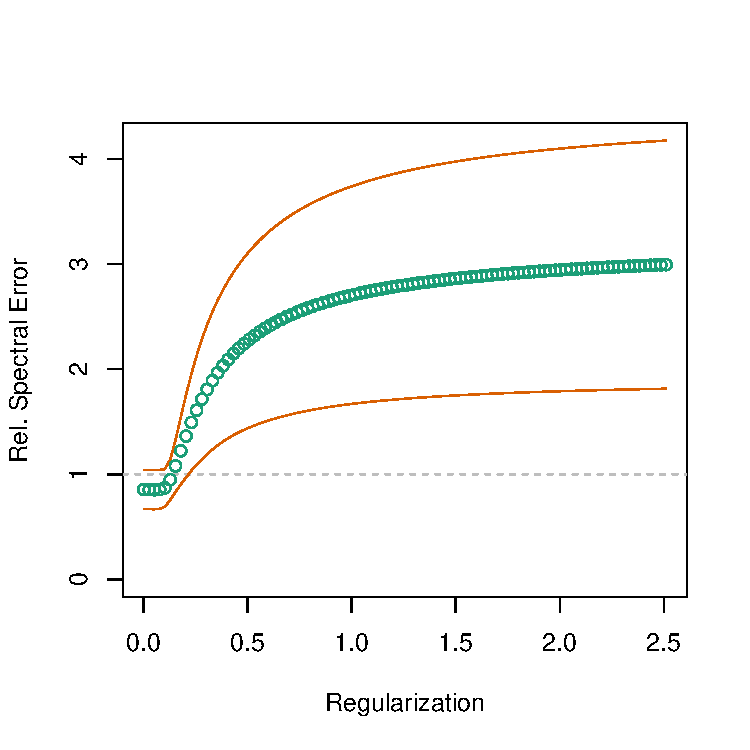
\includegraphics[scale=0.34]{plots/estimation-spec-s0-p020}}
  }
  \subfigure[$m/\mu = 0.2$ and $s = 4$.]{
    \makebox{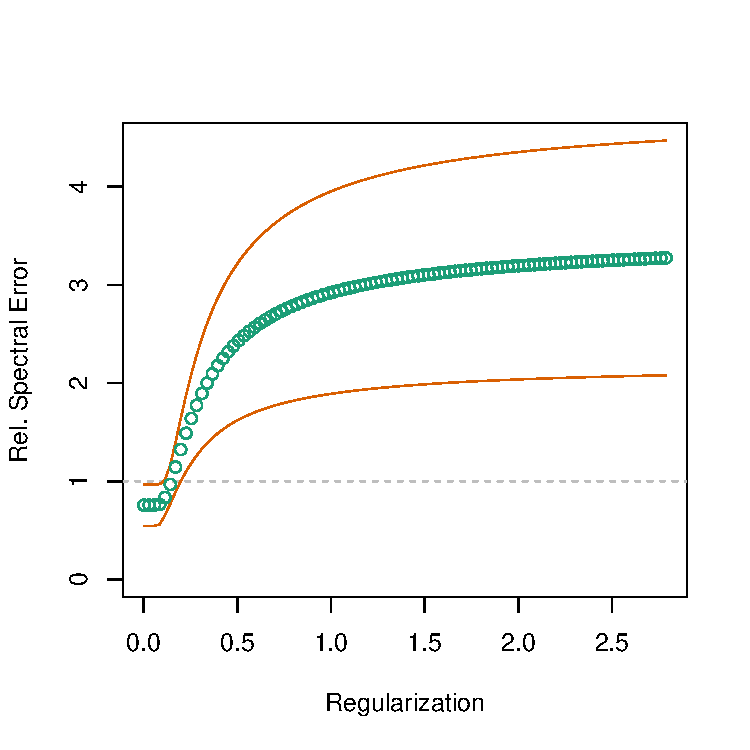
\includegraphics[scale=0.34]{plots/estimation-spec-p020}}
  }
  \subfigure[$m/\mu = 0.2$ and $s = 32$.]{
    \makebox{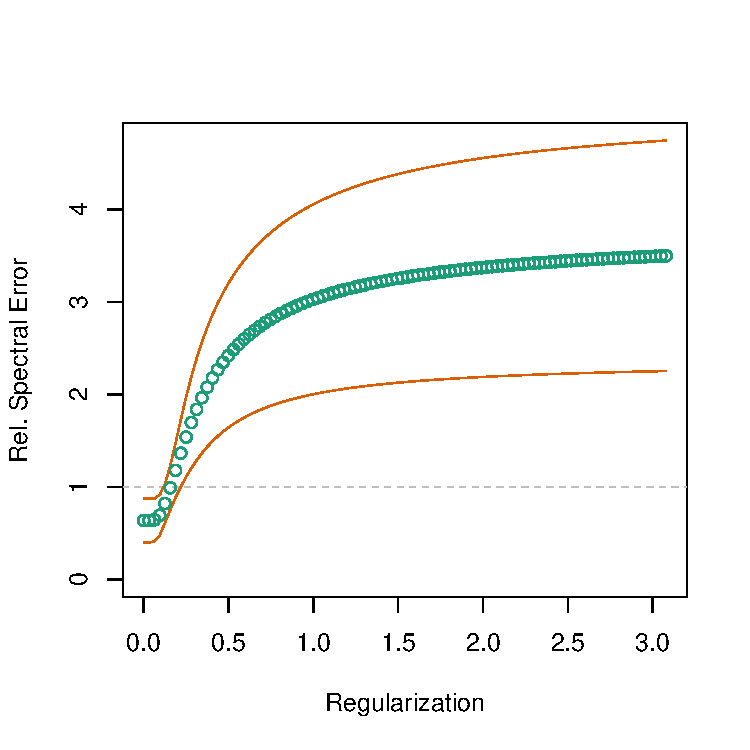
\includegraphics[scale=0.34]{plots/estimation-spec-s32-p020}}
  } \\
  \subfigure[$m/\mu = 2.0$ and $s = 0$.]{
    \makebox{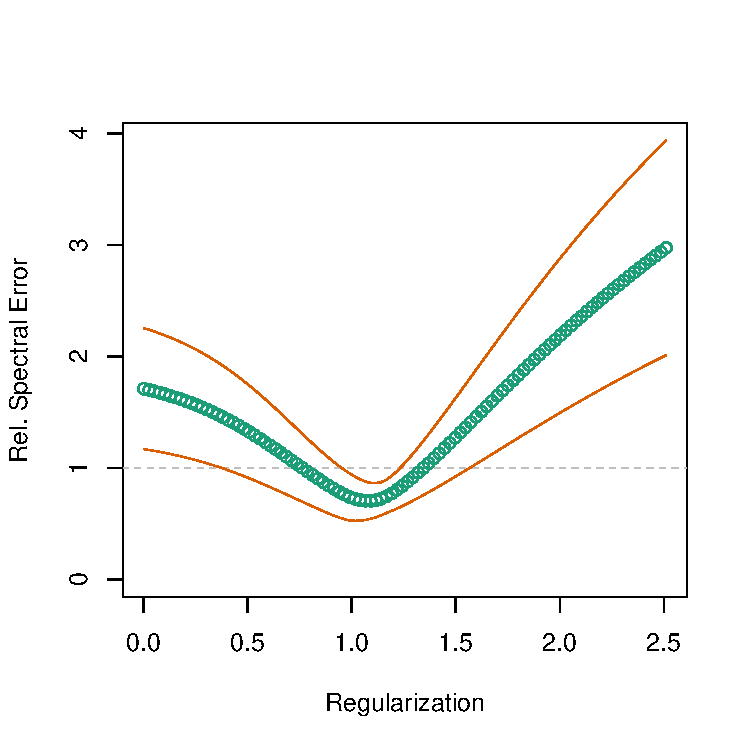
\includegraphics[scale=0.34]{plots/estimation-spec-s0-p200}}
  }
  \subfigure[$m/\mu = 2.0$ and $s = 4$.]{
    \makebox{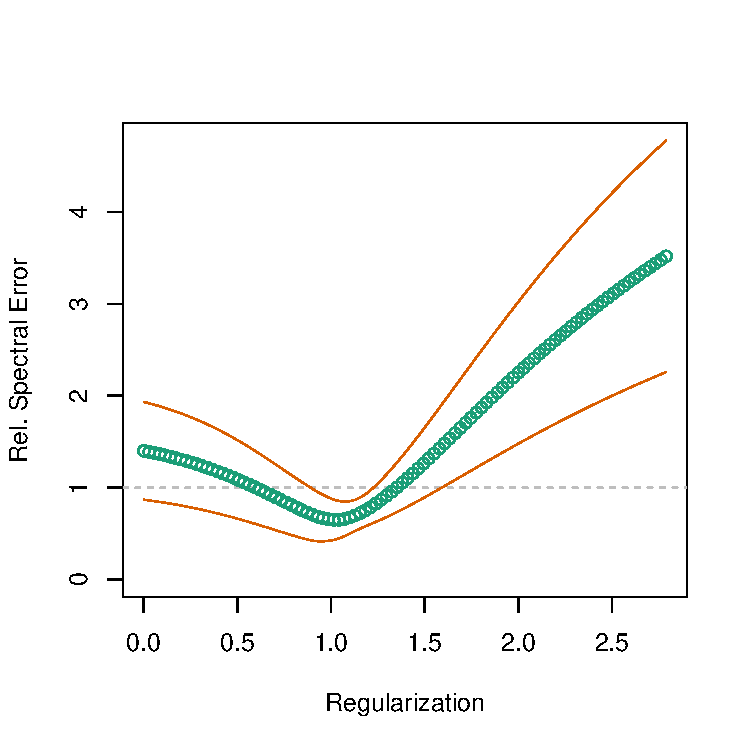
\includegraphics[scale=0.34]{plots/estimation-spec-p200}}
  }
  \subfigure[$m/\mu = 2.0$ and $s = 32$.]{
    \makebox{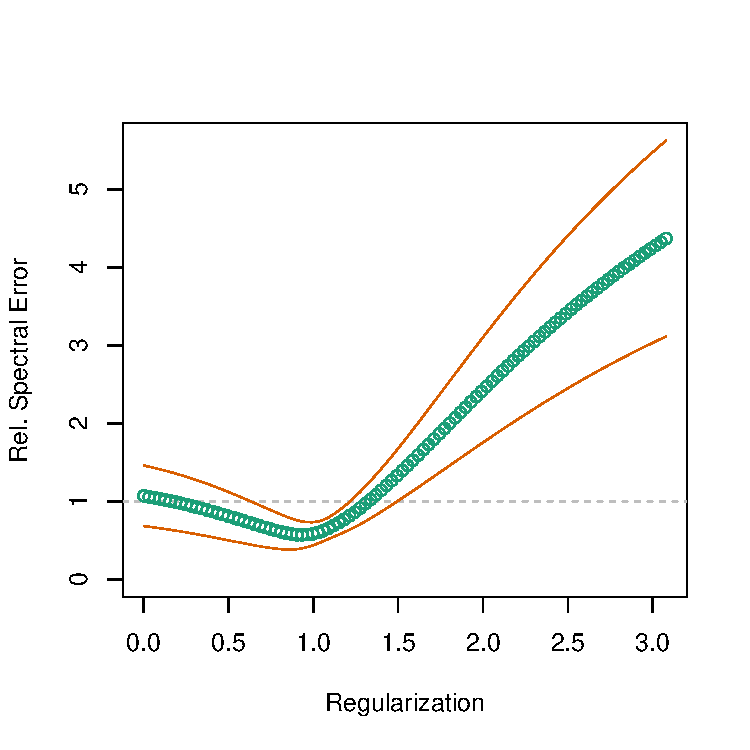
\includegraphics[scale=0.34]{plots/estimation-spec-s32-p200}}
  }
  \vspace{-1em}
\caption{Regularization performance, as measured with the relative 
spectral norm error, versus the (normalized) regularization parameter 
$\eta / \bar \tau$.
Shown are plots for various values of the (normalized) number of edges, 
$m/\mu$, and the edge-swap parameter, $s$.
Recall that the regularization parameter in the regularized 
SDP~(\ref{eqn:mo-reg-sdp}) is $1/\eta$, and thus smaller values along the 
X-axis correspond to stronger regularization.}
\label{fig:perf-spec}
\end{figure}



